\documentclass[12pt]{beamer}\usepackage[]{graphicx}\usepackage[]{color}
%% maxwidth is the original width if it is less than linewidth
%% otherwise use linewidth (to make sure the graphics do not exceed the margin)
\makeatletter
\def\maxwidth{ %
  \ifdim\Gin@nat@width>\linewidth
    \linewidth
  \else
    \Gin@nat@width
  \fi
}
\makeatother

\definecolor{fgcolor}{rgb}{0.345, 0.345, 0.345}
\newcommand{\hlnum}[1]{\textcolor[rgb]{0.686,0.059,0.569}{#1}}%
\newcommand{\hlstr}[1]{\textcolor[rgb]{0.192,0.494,0.8}{#1}}%
\newcommand{\hlcom}[1]{\textcolor[rgb]{0.678,0.584,0.686}{\textit{#1}}}%
\newcommand{\hlopt}[1]{\textcolor[rgb]{0,0,0}{#1}}%
\newcommand{\hlstd}[1]{\textcolor[rgb]{0.345,0.345,0.345}{#1}}%
\newcommand{\hlkwa}[1]{\textcolor[rgb]{0.161,0.373,0.58}{\textbf{#1}}}%
\newcommand{\hlkwb}[1]{\textcolor[rgb]{0.69,0.353,0.396}{#1}}%
\newcommand{\hlkwc}[1]{\textcolor[rgb]{0.333,0.667,0.333}{#1}}%
\newcommand{\hlkwd}[1]{\textcolor[rgb]{0.737,0.353,0.396}{\textbf{#1}}}%
\let\hlipl\hlkwb

\usepackage{framed}
\makeatletter
\newenvironment{kframe}{%
 \def\at@end@of@kframe{}%
 \ifinner\ifhmode%
  \def\at@end@of@kframe{\end{minipage}}%
  \begin{minipage}{\columnwidth}%
 \fi\fi%
 \def\FrameCommand##1{\hskip\@totalleftmargin \hskip-\fboxsep
 \colorbox{shadecolor}{##1}\hskip-\fboxsep
     % There is no \\@totalrightmargin, so:
     \hskip-\linewidth \hskip-\@totalleftmargin \hskip\columnwidth}%
 \MakeFramed {\advance\hsize-\width
   \@totalleftmargin\z@ \linewidth\hsize
   \@setminipage}}%
 {\par\unskip\endMakeFramed%
 \at@end@of@kframe}
\makeatother

\definecolor{shadecolor}{rgb}{.97, .97, .97}
\definecolor{messagecolor}{rgb}{0, 0, 0}
\definecolor{warningcolor}{rgb}{1, 0, 1}
\definecolor{errorcolor}{rgb}{1, 0, 0}
\newenvironment{knitrout}{}{} % an empty environment to be redefined in TeX

\usepackage{alltt}%
\setbeamersize{text margin left=0.5cm, text margin right=0.5cm}

\usepackage{alltt}%
\usetheme[background=light]{metropolis} 
\usecolortheme{seahorse}

\usepackage[utf8]{inputenc}%


\usepackage[normalem]{ulem}%strikeout
 

% graphics
%% Figures %%%%%%%%%%%%%%%%%%%%%%%%%%%%%%%%%%%%%%%%%%%%%%%%%%
\usepackage{graphicx}
\usepackage{xcolor}%for color mixing

\usepackage{amsmath}%
\usepackage{amsfonts}%
\usepackage{amssymb}%
\usepackage{graphicx}

\usepackage{tikz}
\usetikzlibrary{calc}

\usepackage{hyperref}

%%%%%%%%%%%%%%%%%%%%%%%%%%%%%%%%%%%%%%%%%%%%%%
%%%%%%%%%%%%%%%%% Doc info %%%%%%%%%%%%%%%%%%%
\title{Model selection in R, part 2}
\subtitle{Information Criteria and statistical inference}
\author{Timoth\'ee Bonnet}
\institute{BDSI / RSB}
\date{\today}

%%%%%%%%%%%%%%%%%%%%%%%%%%%%%%%%%%%%
\IfFileExists{upquote.sty}{\usepackage{upquote}}{}
\begin{document}



\begin{frame}
  \begin{quote}
  ``Data dredging (also called data snooping, data mining, post hoc data analysis)
should generally be avoided, except in (1) the early stages of exploratory work
or (2) after a more confirmatory analysis has been done. In this latter case,
the investigator should fully admit to the process that led to the post hoc
results and should treat them much more cautiously than those found under
the initial, a priori, approach."
  \end{quote}

Burnham and Anderson, 2002, Model Selection and Multimodel Inference: A Practical Information-theoretic Approach

\end{frame}
%%%%%%%%%%%

\begin{frame}
\maketitle
\end{frame}
%%%%%%%%%%%


\AtBeginSection[]
{
  \begin{frame}<beamer>
    \Large
    \frametitle{}
    \tableofcontents[currentsection,hideothersubsections,subsectionstyle=hide]% down vote\tableofcontents[currentsection,currentsubsection,hideothersubsections,sectionstyle=show/hide,subsectionstyle=show/shaded/hide]
  \end{frame}
}

\begin{frame}[standout]{If you get bored:}
Scroll down the slides and find "Challenge exercises".
\end{frame}

%%%%%%%%%%%%%%%%%%%%%%%%%%%%%%%%%%%%%%%%%%%%%%%%%%%%%%%%%%%%%%%%%%%
%%%%%%%%%%%%%%%%%%%%%%%%%%%%%%%%%%%%%%%%%%%%%%%%%%%%%%%%%%%%%%%%%%%

\section{Model selection and automation}

\begin{frame}{Reminder: Why model selection}

  \begin{exampleblock}{}
    \begin{itemize}
      \item Adding predictors increases fit to the response, in the current data
      \item But too many predictors:
        \begin{itemize}
          \item DECREASE fit in new data (from the same population)
          \item Hinder biological interpretation
          \item Increases esimtation uncertainty (larger SE and p-values)
        \end{itemize}
      \item Model selection aims to balance fit and generalisation 
    \end{itemize}
  \end{exampleblock}
\end{frame}
%%%%%%%%%%%

\begin{frame}{Information criteria}

\begin{exampleblock}{Akaike information criterion (AIC)}
  \begin{itemize}[<+->]
    \item AIC = 2$\times$Number of parameters - 2$\times \log(\text{model likelihood})$
    \item Smaller is better
    \item Only relative measure, no absolute meaning
    \item In R: \texttt{AIC(model)}
  \end{itemize}
\end{exampleblock}

\end{frame}
%%%%%%%%%%%

\begin{frame}{Practice: reminder AIC}

\begin{center}
  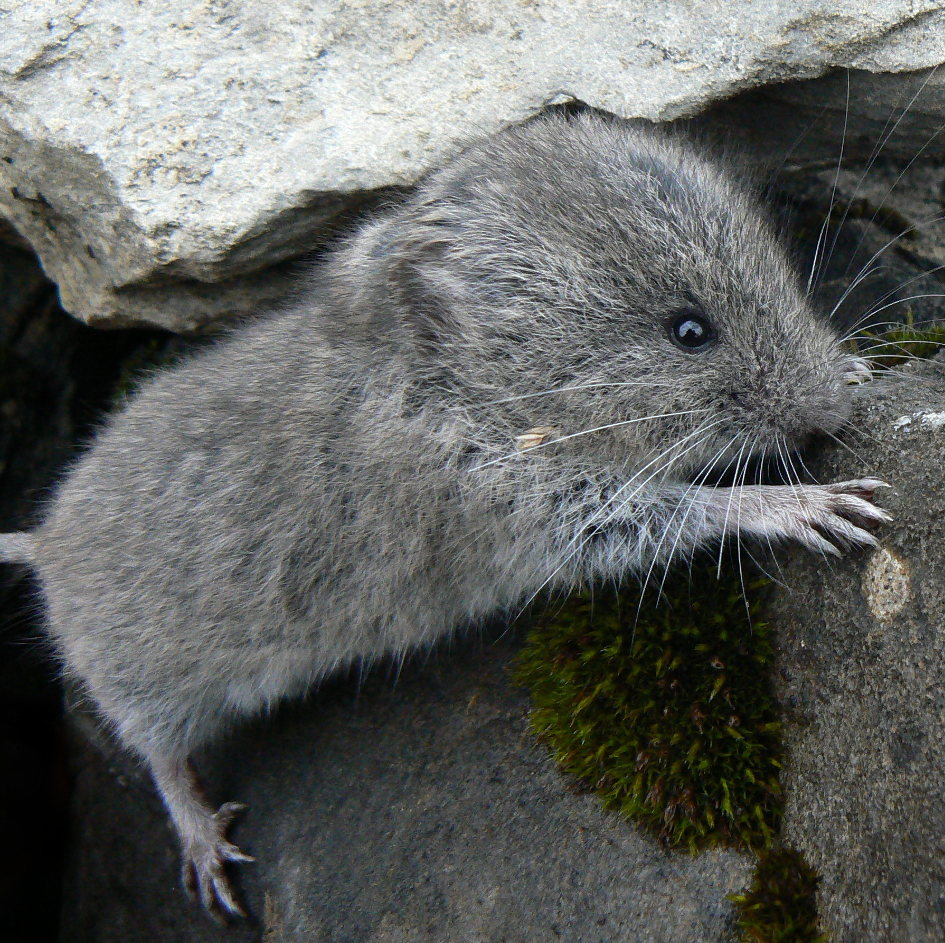
\includegraphics[width=0.4\textwidth]{Figures/vole}
\end{center}

Load \texttt{VoleWeight.csv}. 

We want to understand what factors explain variation in individual body weight. Compare a few (plausible) models with AIC.

\end{frame}
%%%%%%%%%%%

\begin{frame}{Different information criteria?}
\begin{alertblock}{2 most important:}
\begin{enumerate}
  \item AICc (\texttt{MuMIn::AICc()})
    \begin{itemize} 
      \item Small sample size correction for AIC
      \item Can always been used instead of AIC
      \item \textbf{Maximizes prediction} (of new data)
    \end{itemize}
    \pause
  \item Bayesian Information Criterion (\texttt{stat::BIC()})
    \begin{itemize}
      \item More penalty per parameter 
      \item Simpler models than AIC / AICc
      \item \textbf{Maximizes consistency} (=effects you find in model selection data likely to be present in new data)
    \end{itemize}
\end{enumerate}
\end{alertblock}

\end{frame}
%%%%%%%%%%%

\begin{frame}{Package \texttt{MuMIn}}
 
\begin{knitrout}\small
\definecolor{shadecolor}{rgb}{0.843, 0.867, 0.922}\color{fgcolor}\begin{kframe}
\begin{alltt}
\hlkwd{install.packages}\hlstd{(}\hlstr{"MuMIn"}\hlstd{)}
\hlkwd{library}\hlstd{(MuMIn)}
\end{alltt}
\end{kframe}
\end{knitrout}

\pause

\begin{exampleblock}{1. AICc}
  \begin{itemize}
    \item AIC is biased for small sample size
    \item AICc (``second-order AIC") when sample size / number of parameters is less than 40
    \item \texttt{MuMIn::AICc()}
  \end{itemize}
\end{exampleblock}

\pause

\begin{alertblock}{2. dredge}
  \begin{itemize}
    \item Automate model selection
    \item Many competing models, some may not make sense
    \item \texttt{MuMIn::dredge()}
  \end{itemize}
\end{alertblock}

\end{frame}
%%%%%%%%%%%

\begin{frame}{Try automated model selection}

Try to use \texttt{dredge()}, with selection based on \texttt{AICc}, to automate model selection on the vole data. Start from a model including all predictors (plus some interactions).

For some reason you first need to run:
\begin{knitrout}\small
\definecolor{shadecolor}{rgb}{0.843, 0.867, 0.922}\color{fgcolor}\begin{kframe}
\begin{alltt}
\hlkwd{options}\hlstd{(}\hlkwc{na.action}\hlstd{=}\hlstr{"na.fail"}\hlstd{)}
\end{alltt}
\end{kframe}
\end{knitrout}


Do you find the same result as on slide 6?

\end{frame}
%%%%%%%%%%%

\begin{frame}{dredge() best practices}

\begin{knitrout}\small
\definecolor{shadecolor}{rgb}{0.843, 0.867, 0.922}\color{fgcolor}\begin{kframe}
\begin{alltt}
\hlkwd{dredge}\hlstd{(}\hlkwc{global.model}\hlstd{= ,}\hlkwc{fixed} \hlstd{= ,}\hlkwc{varying}\hlstd{= ,}\hlkwc{subset}\hlstd{= ,}\hlkwc{rank}\hlstd{=)}
\end{alltt}
\end{kframe}
\end{knitrout}

\begin{itemize}[<+->]
  \item \texttt{global.model} makes sense; not too complicated
  \item \texttt{fixed} coefficients across models
  \item \texttt{subset} and \texttt{varying} for more complex subset of models to test
  \item \texttt{rank=AICc} or \texttt{BIC}; decide before you look!
\end{itemize}

\end{frame}
%%%%%%%%%%%


\begin{frame}[fragile]{Practice: constrain dredge}

Still using the vole data, use dredge to select among models of the effects of humidity and temperature while controling for sex and age. Use the arguments \texttt{fixed} or \texttt{varying}. 

Also check the difference between AICc and BIC based model selection.

Your starting model is:
\begin{knitrout}\small
\definecolor{shadecolor}{rgb}{0.843, 0.867, 0.922}\color{fgcolor}\begin{kframe}
\begin{alltt}
\hlstd{m0} \hlkwb{<-} \hlkwd{lm}\hlstd{(Weight} \hlopt{~} \hlstd{Sex}\hlopt{*}\hlstd{Age} \hlopt{+} \hlstd{humidity}\hlopt{*}\hlstd{temperature} \hlopt{+}
           \hlkwd{as.factor}\hlstd{(Year) ,} \hlkwc{data} \hlstd{= voles)}
\end{alltt}
\end{kframe}
\end{knitrout}



\end{frame}
%%%%%%%%%%%



\section{Model selection and causal inference}

\begin{frame}{Principle of model selection based causal inference}
\begin{exampleblock}{}
  \begin{enumerate}[<+->]
    \item List biological hypotheses
    \item Define statistical models corresponding to hypotheses
    \item Importantly, the models do not have to be nested or look the same
    \item (AIC/)BIC model selection
    \item Which models/hypotheses do better? Is one clearly best? 
    \item Do NOT trust parameter estimates/p-values (need confirmatory model)
  \end{enumerate}
\end{exampleblock}
\end{frame}
%%%%%%%%%%%

\begin{frame}[fragile]{Practice: Competing hypotheses}



How does respiration rate scale with body mass in mammals? For a while researchers fought over different hypotheses: respiration could increase as a function of $mass^{2/3}$, as a function of $mass^{3/4}$ or as a function of $log(mass)$; while maybe the shape of the animals played a role. Let's find out!

Load \texttt{metabo.csv} and compare models through AIC or BIC selection.

NB: you can fit exponents of a predictors using the function \texttt{I()}. For instance, for the exponent 0.5 of x:
\begin{knitrout}\small
\definecolor{shadecolor}{rgb}{0.843, 0.867, 0.922}\color{fgcolor}\begin{kframe}
\begin{alltt}
\hlkwd{lm}\hlstd{(y} \hlopt{~} \hlkwd{I}\hlstd{(x}\hlopt{^}\hlstd{(}\hlnum{1}\hlopt{/}\hlnum{2}\hlstd{)))}
\end{alltt}
\end{kframe}
\end{knitrout}

\end{frame}
%%%%%%%%%%%


\begin{frame}{Do not choose statistical framework after applying them; do not trust model estimate after model selection}
\begin{figure}
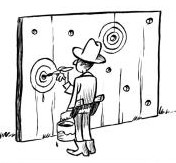
\includegraphics[width=0.5\textwidth]{Figures/dirk-jan-hoek}
\caption{Null-hypothesis testing after model selection \copyright Dirk Jan-Hoek}
\end{figure}
\end{frame}
%%%%%%%%%%%

\begin{frame}{Practice}

Tell what drives the increase in number of babies in \texttt{babies.csv}. Compare AICc vs. BIC model selection. 


\end{frame}
%%%%%%%%%%%

\begin{frame}[fragile]{Practice (challenge): P-values and model selection}
\footnotesize
When a predictor is independent of the response there is a 5\% probability to find a p-value below 0.05 (that's a false positive). But it does not work if we do model selection first! Create a for-loop based on the code below to look at the distribution of p-values after model selection.

\begin{knitrout}\small
\definecolor{shadecolor}{rgb}{0.843, 0.867, 0.922}\color{fgcolor}\begin{kframe}
\begin{alltt}
\hlstd{nobs} \hlkwb{<-} \hlnum{60}
\hlstd{mainpredictor} \hlkwb{<-} \hlkwd{rnorm}\hlstd{(nobs)}
\hlstd{control1} \hlkwb{<-} \hlkwd{rnorm}\hlstd{(nobs) ; control2} \hlkwb{<-} \hlkwd{rnorm}\hlstd{(nobs)}
\hlstd{control3} \hlkwb{<-} \hlkwd{rnorm}\hlstd{(nobs) ; control4} \hlkwb{<-} \hlkwd{rnorm}\hlstd{(nobs)}
\hlstd{control5} \hlkwb{<-} \hlkwd{rnorm}\hlstd{(nobs) ; response} \hlkwb{<-} \hlkwd{rnorm}\hlstd{(nobs)}
\hlstd{mfull} \hlkwb{<-} \hlkwd{lm}\hlstd{(response} \hlopt{~} \hlstd{mainpredictor} \hlopt{+}
      \hlstd{control1}\hlopt{*}\hlstd{control2}\hlopt{*}\hlstd{control3} \hlopt{+} \hlstd{control4}\hlopt{*}\hlstd{control5)}
\hlstd{modall} \hlkwb{<-} \hlkwd{dredge}\hlstd{(mfull,} \hlkwc{fixed} \hlstd{=} \hlstr{"mainpredictor"}\hlstd{)}
\hlkwd{summary}\hlstd{(}\hlkwd{get.models}\hlstd{(modall,} \hlnum{1}\hlstd{)[[}\hlnum{1}\hlstd{]])}\hlopt{$}\hlstd{coefficients[}\hlnum{2}\hlstd{,}\hlnum{4}\hlstd{]}\hlcom{#the pvalue}
\end{alltt}
\end{kframe}
\end{knitrout}


\end{frame}
%%%%%%%%%%%


\begin{frame}{Summary: Model selection and inference}

  \begin{exampleblock}{}
    \begin{itemize}
      \item AIC best for exploratory / predictive models
      \item BIC best for robust / consistent models
      \item AIC/BIC alone can be used for causal inference if models are all meaningful competing hypotheses
      \item After AIC/AICc selection p-values are wrong
      \item Parameter estimates, p-values and standard errors MUST be computed on new data (Confirmatory model)
    \end{itemize}
  \end{exampleblock}
  
\end{frame}

%%%%%%%%%%%%%%%%%%%%%%%%%%%%%%%%%%%%%%%%%%%%%%%%%%%%%%%%%%%%%%%%%



\begin{frame}{Challenge!}

What drives bird abundance (ABUND) in \texttt{loyn.csv}?

\end{frame}
%%%%%%%%%%%


\begin{frame}{Challenge!}

\textbf{How do differences in AIC between nested models scale with F-statistic p-values for the extra predictor? Use some simulations to explore the issue.}

\end{frame}
%%%%%%%%%%%

\begin{frame}[standout]{Take-home messages}
\vspace{-0.5cm} \large
\begin{exampleblock}{}
  \begin{enumerate}[<+->] 
    \item Model selection biases estimates/p-values; confirm with new data
    \item Model selection alone can be used for inference; needs careful choice of models
    \item Choose method before analysis (AIC or BIC or confirmatory model?)
  \end{enumerate}
\end{exampleblock}

\end{frame}
%%%%%%%%%%%

\begin{frame}{Want to know more?}

\begin{alertblock}{AIC vs. BIC vs. P-values:}
\begin{itemize}
  \item \textbf{``AIC does everything": }Burnham and Anderson, 2002, Model Selection and Multimodel Inference: A Practical Information-theoretic Approach
  \item \textbf{``Sometimes BIC works better":} Brewer \& al. The relative performance of AIC, AICc and BIC in the presence of unobserved heterogeneity. Methods in Ecology and Evolution. 2016, 7, 679–692.
  \item \textbf{``Your goal matters in the choice between AIC, BIC, p-values...:"} Aho \& al. A graphical framework for model selection criteria and significance tests: Refutation, confirmation and ecology. Methods in Ecology and Evolution. 2017;8:47–56.
\end{itemize}
\end{alertblock}

\end{frame}
%%%%%%%%%%

\begin{frame}[standout]{}
  \begin{exampleblock}{Before you leave:}
  \begin{enumerate}
    \item Write one thing you liked and one you disliked on a sticky note
    \item Presence sheet! (HDR career development framework)
    \item Email address to join the Slack channel 
    \item Past workshops at \url{https://timotheenivalis.github.io/RSB-R-Stats-Biology/} 
  \end{enumerate}
\end{exampleblock}
\end{frame}

\end{document}
